\section{多次反射处理方法的前景}
\label{sec:5.6}

要改善压制多次波的能力,我们就得力争比较好地描述其特征,麻烦的是实际模型总是
有许多的组成因素。在丰富的文献中几乎没多少理论已经对日常的生产实践有很大影响,我
把那些不成功的理论分成两类:
\begin{enumerate}
\item 试图以统计方法解决每个问题,把空间关系过分简化了的那些理论;
\item 试图以数学物理方法解决每个问题,把资料的不完全性质和干扰性质过分简化了
的那些理论。
\end{enumerate}

对于进入地球物理领域的原子核物理学家、天体衡理学家和数学家来说,多次反射是一
个很合适的题目。那些愿意接受挑战、力图坚持理论联系生产实践的人们学会谦虚谨慎一些
就能得到报偿。我愿现在告诫你们,在这节中我始终还未曾把它们拉扯在一起!

本节将提出两种处理办法,这二者均注重几何方法和统计方法,两种办法都是新方法而
且没经过多少检验,不论它们如何能起良好作用,我想你们会发现它们对解决这个任务总是
有所启发的。

第一种方法称作共中心点倾斜叠加(CMP slant stack),这是其中简单的一种方法,
它将资料变换成这样一种彤式:其中所有炮检距上的记录道均是模仿简单的一维零炮检距模
型,关于该种模型的文献在数学物理和统计学中是很广泛的。

第二种方法是以置换阻抗(replacement inpedance)概念为基础,设计它的意图是为了
适应近地面的快速横向变化。用假想的海上环境条件最容易解释这种方法的意义,其中产生
的唯一困难就是海底反射率之横向变化。方法的基本思想是将定向的炮点与定向的检波点向
下延拓至不多不少正好在海底之下,然后经由一卜具有零值海底反射系数的置换介质向上延
拓;这种处理过程不会消除所有的多次反射,但是它应能消除最令人恼火的一些多次波。

\subsection{以倾斜叠加方法变换至一维情形}
\label{sec:5.6.1}

关于多次反射的一维模型,现在有丰富的文献,一些著者发展了波动传播理论的许多分
支方面的工作,另一些著者则从简化传播模型开始着手,发展了信息论的许多分支方面的工
作。这些一维理论总是被认为只能应用于零炮检距情形,其实,我们将会看到,以倾斜叠加
作为工具是可以使所有其他炮检距情形都能进入一维问题领域的。



% \begin{figure}[H]
% \centering
% 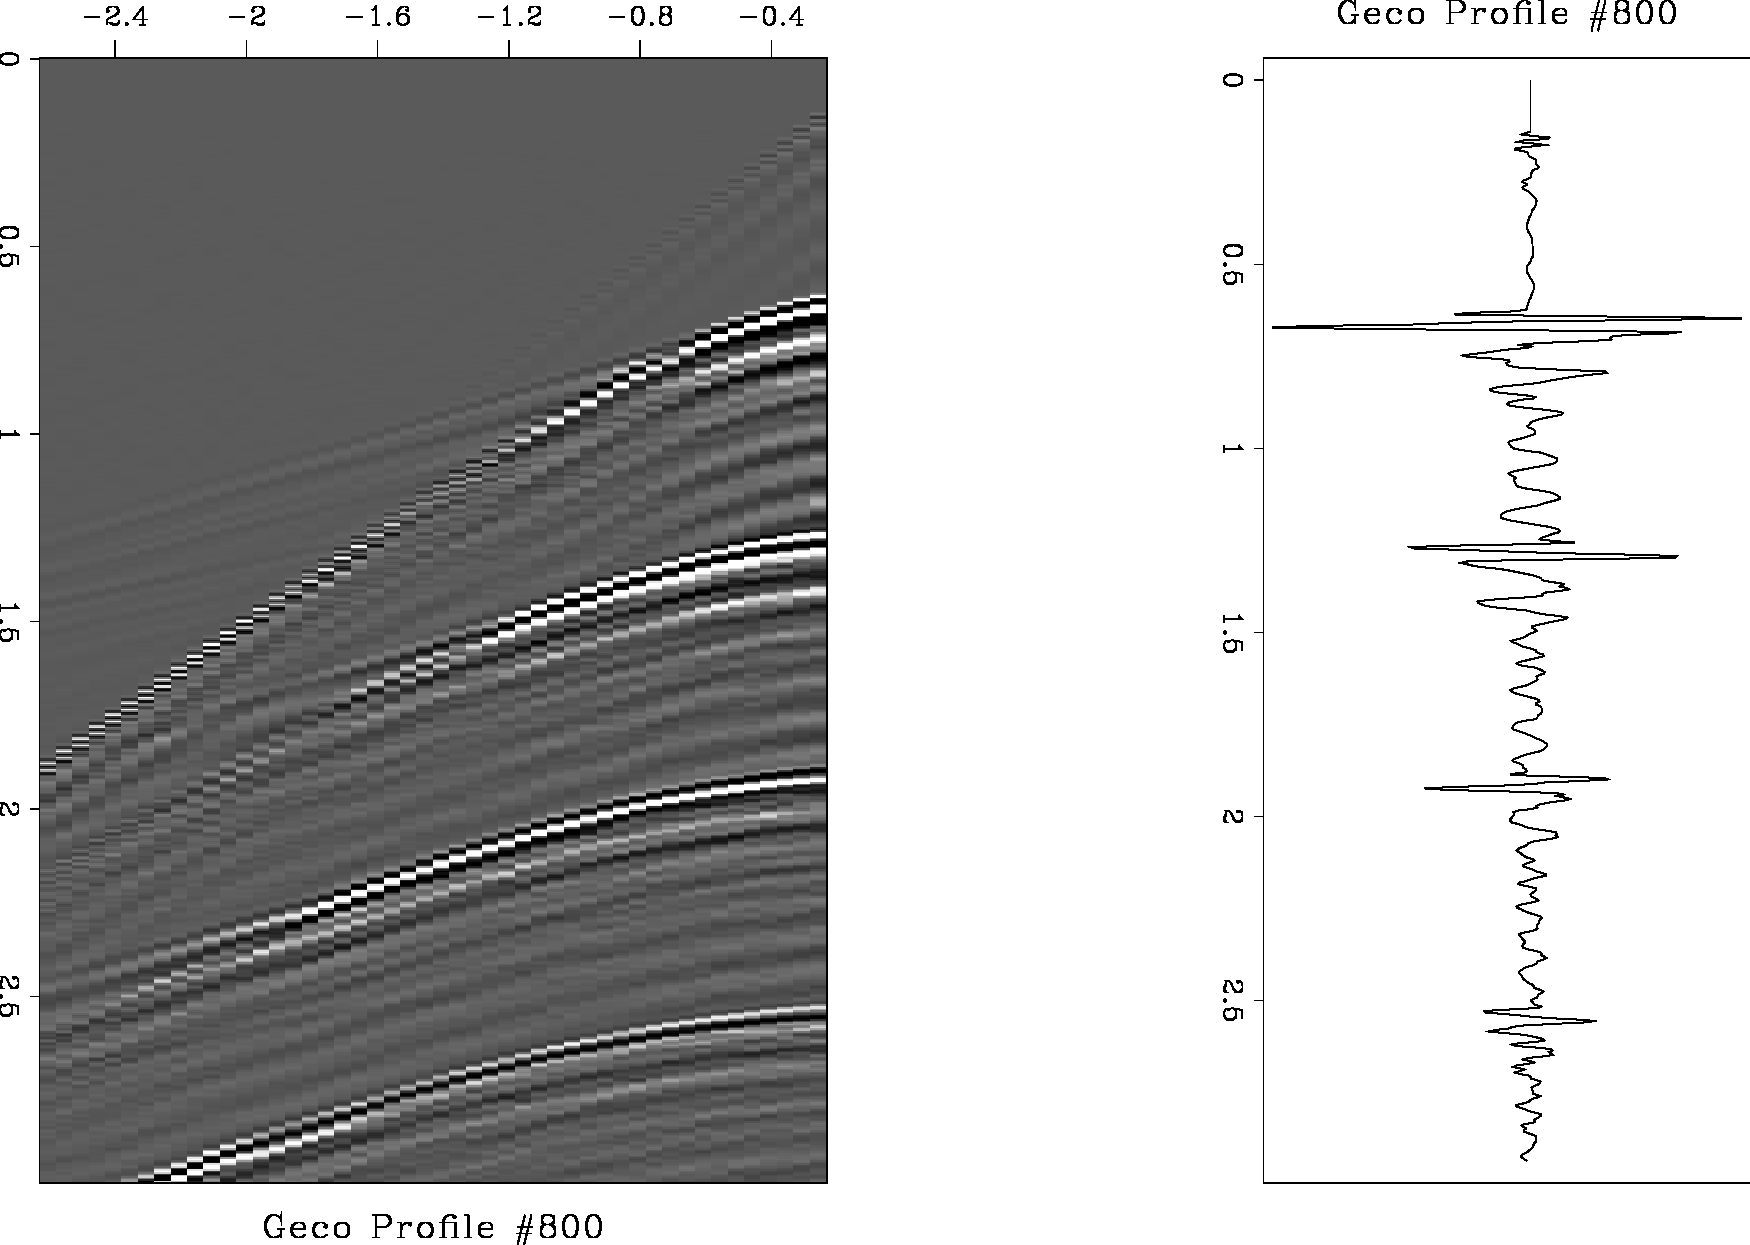
\includegraphics[width=0.65\textwidth]{mltp/multiple}
% \caption[multiple]{挪威的多次反射海上剖面。左侧是经过放大的近炮点记录道(据挪威GECO公司)
% }
% \label{fig:mltp/multiple}
% \end{figure}

% \subsection{常规数据处理中的反褶积}
% \label{sec:5.5.2}

% 在图\ref{fig:mltp/multiple}中,海水层深度比典型石油勘探深度要大些,图\ref{fig:mltp/gsidecon}与图\ref{fig:mltp/pns}才是更典型的情形。在图\ref{fig:mltp/gsidecon}中,海水层深度浅到不可能辨别出反射了。就陆地资料来说,风化层底部
% 通常很浅且模糊不清,以致一般不可能识别出单独的反射。“浅”这个字眼R用于多次反射
% 时是限定只指反射记录变化很迅速,以至没办法钯它们彼此明显区别开来。

% \begin{figure}[H]
% \centering
% 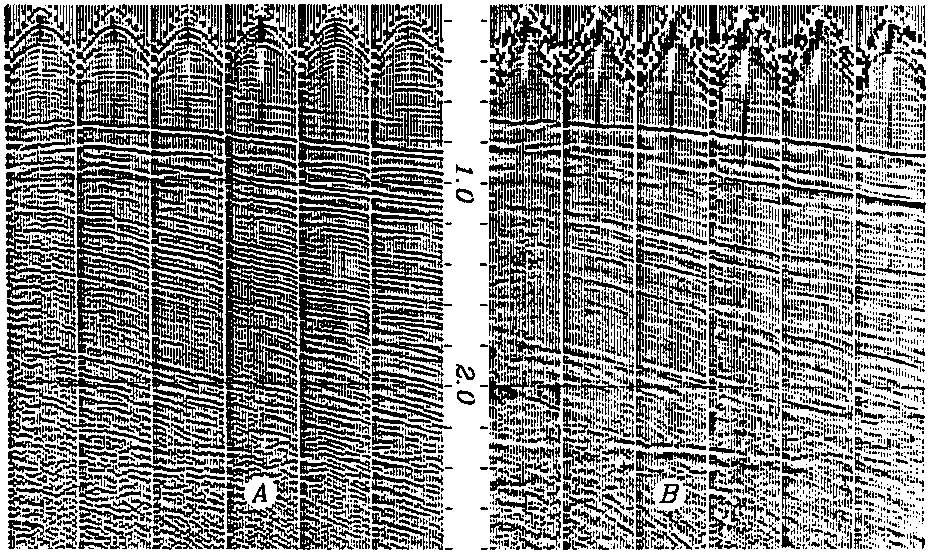
\includegraphics[width=0.65\textwidth]{mltp/gsidecon}
% \caption[gsidecon]{
% 反褶积之前(左图)和反褶积之后(右图)的野外剖面(GSI公司公布,
% 公元1965年)
% }
% \label{fig:mltp/gsidecon}
% \end{figure}

% \begin{figure}[H]
% \centering
% 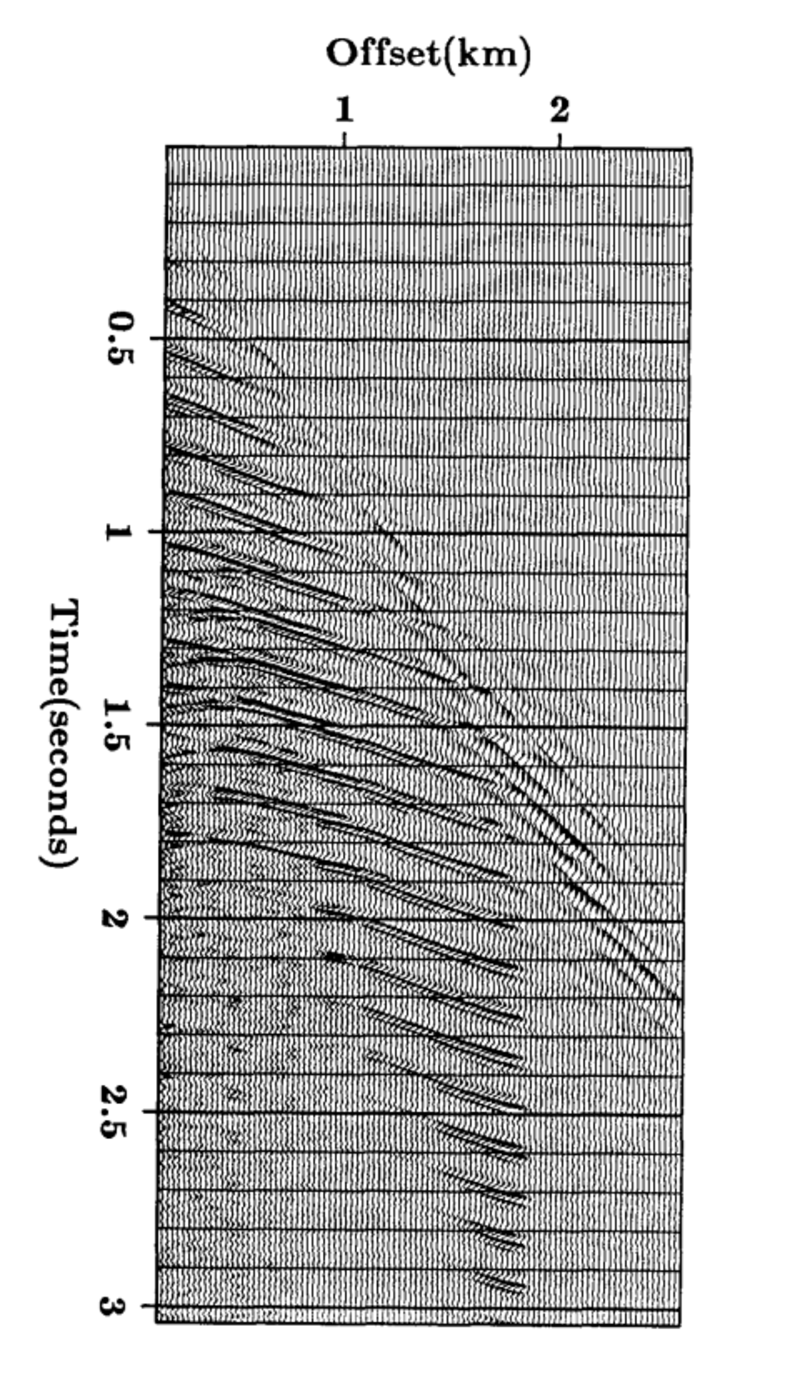
\includegraphics[width=0.65\textwidth]{mltp/pns}
% \caption[pns]{
% 北海剖面(西方地球物理公司)。具有周期大约为90毫秒
% 之很强的交混回响,它们是海底的多次反射。注意,最强
% 的信号出现在随时间增长而增大的炮检距上,这是因为最强
% 的多次波常常在临界角上出现。在船后1.8公里处交混回响
% 强度突然减低,这是暗示在该点处的海底有突然变化。
% }
% \label{fig:mltp/pns}
% \end{figure}

% 关于反褶积这个题目,统计学家已经写了一大堆丰富文献了,对于他们来说,这问题实际
% 是一个估计震源波形而不是消除多次反射的问题。在一定的数学极限之内可使震源波形问題
% 等价于多次反射问题,当混响只限于炮点或
% 检波点周围很小的物理体积之内、诸如在土壤
% 层之内时,这种极限就能成立。震源波形与多
% 次反射问题之所以能够在这神情形下等价,原
% 因就在于炮点产生的下行波不但对于炮点本身
% 来说是固有的,而且也包括了局部土壤层的共
% 振。在反射地震学中,虚反射这个词是指震源
% 的反射再加上来自地面的反射(或有时来自风
% 化层底部),因为震源非常接近这些反射面,
% 所以我们往往把虚反射也看成是震源波形的一部分。

% 关于垂直入射情形下的多次反射模型,也
% 有广泛的文献。在波动传播理论工作者当中,
% 把消除多次波称作反演问题。看起来,要使反
% 演理论能应用于实际问题。必须同可处理爆烊
% 波形未知、频谱性质欠缺问题的分析方法结合起来才行。

% 常规生产性的反褶积(图\ref{fig:mltp/gsidecon})有许多
% 种导忠方法积解释,我将以简单的术语来阐述
% 那些我相信是反褶积之本质的一些问题。每个
% 地震记录都有一个谱,该谱是许多因素产生的
% 结果,某些因素具有基本意义,另一些兜j是不增大的炮检距上,这是因为最强的多次波常常在临界角上
% 重要的。当迆震记录正好因某种近地表现象而
% 产生共鸣震荡时,这就使人感到麻烦了。反褶积
% 基本上是这么一种处理:测定出强共鸣震荡,然后设计一种滤波处理去皮制它们。所设
% 计的滤波具有一种特定的谱,它应大致等于原始数据之谱的倒数,因而,滤波的输出大致为
% 白噪(所有频率成分均相等)。从最早期开始,地震学家就已经发现反射地震数据在10至
% 100赫兹频带之外很少有多大意义,所以采取的最后一个步骤就是将该频带范围之外的频率
% 成分均消除。(对大多数地震学家来说,关于输出的谱应为白噪的假设看来是一稗不得已的
% 假设,但是实践通常都表明,比起从原始数据来解释地层映象,那它还是更可取的)。

% 关于反褶积在实践中为什么成功还有另一种非数学的解释,这就是,它使谱逐道相等了,
% 它实现了各个谱的均衡(Tufekcic等,1981)。不但迆震记录因某科近地表现象而出现共振
% 是件烦扰的事,而且波谱随近地表条件之逐点变化而出现逐道变化,更是一件令人头痛的
% 事,变化的波谱使得时差的测定很难进行。要注意,以上所述的常规生产性反褶积处理就是
% 将谱均衡(spectral balancing)作为一种副产品包括在内的。图\ref{fig:mltp/pns}所示就是需要进行
% 谱均衡的数据。

% 上述对反褶积及其为何能起作用的解释不同于大多数地球物理文献中所作的解释,通常
% 总是用多次反射可预测而一次反射不可预测来解释反褶积。在《地球物理数据处理基础》一
% 书中指出过如何预测多次反射,它们不是采用严格的褶积模型,而只不过是近似迆采用该模
% 型来预测多次反射。只有当交混回响全部存在于浅层中时,基于褶积模型的预测才起最佳作
% 用。这时,交混回响丨象是一个震源波形。

% 心血管研究须很好地与日常实践结合起来,而肺功能研究则否。我认为这点与下述事实
% 可相比拟:偏移理论与速度理论是生产实践的良好指南,而反褶积理论则不然。理论与实践
% 之间留有较大之空白,意味着还存在有某种有待认识的事物。某些领域很难直接着手解决,
% 在这些领域中,你必须循着更迂迴的间接途径前进,学生会被这弄糊涂,而缺乏耐心的人则
% 会感到混乱,但是,仅此途径,别无他法。欲悉详情,可阅ZioIkowski(1984)的著作。

% 下面将用少量篇幅指出,采用井中检波器的陆地资料进一步证实震源波形主耍就是近地
% 表交混回响;然后离开褶积模型,转而讨论其它。

% \subsection{垂直地震剖面(VSP)}
% \label{sec:5.5.3}

% 地震学家总是欢迎垂直地震剖面的额外信息。VSP是震源在地面、由井中检波器记录所
% 得地震记录的某种组合,诸如岩屑和电测井等常规以井为基础的观测都是记录局部信息,影
% 响所及范围距井壁不过几公分。把地层考虑为水平成层倒是不错,但就是距井壁为某种未知
% 距离之处这种理想化情形并不成立。反射勘探地震学尽管离钻井观测的“可靠真理”还差得
% 远,仍能提供关于横向连续性所需要的信息,但是地面观测反射资料既受分辨能力限制,又
% 有其他不肯定性响影。VSP提供中等比例尺度的信息,而且还为地面地震方法提供一种标定
% 办法,可惜的是,VSP方法的费用昂贵,因而我们很难得到VSP数据。

% 关于VSP这个题目已有若干专著和许多研究论文(见Gal'perin,1974及Balch等,1982),
% 在这里我们将只考虑一个VSP记录,以便得出震源波形及多次反射的某些概念。图\ref{fig:mltp/vspl}所
% 示VSP剖面取自典型的陆地区域,多次反射影响不如本章其他处所示海上资料那么严重。图
% \ref{fig:mltp/vspl}中最早到达的波至是一次下行波。下行波旅行时间随深度而増大,时距曲线之斜率给
% 出向下速度分量。在第一个下冇波到达以后,你可见有更多的具有相同速度之下行波。上行
% 波具有与下行波符号相反的斜率,这些波在图\ref{fig:mltp/vspl}内亦明显可见。
% \begin{figure}[H]
% \centering
% 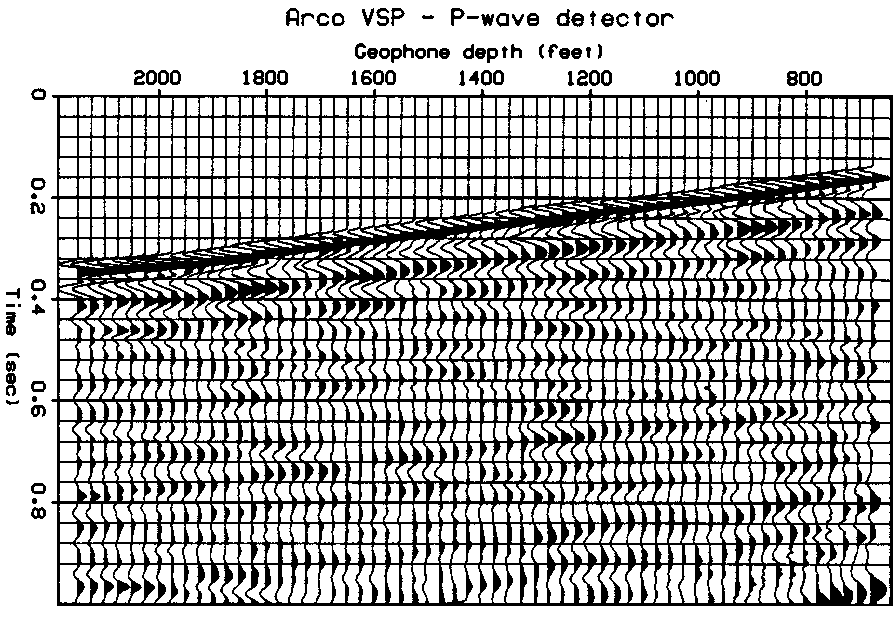
\includegraphics[width=0.65\textwidth]{mltp/vspl}
% \caption[vspl]{
% 垂直地震剖面。震源位于钻孔附近地表面,水平轴为接收器深度,垂直轴为
% 从零至一秒的旅行时间。振幅均按$t^{1.5}$作比例标定(ARCO公司)
% }
% \label{fig:mltp/vspl}
% \end{figure}

% 由于晚到的反射弱于早到的硖,地震资料在进行显示之前通寧要辨时间而加以比例
% 标定,关于什么比例标定最好的问题,无论在理论上或实践中都没有什么通用规定。通常,我
% 发现按$t^2$进行标定可使反射资料令人满意(见\ref{sec:4.1}节)。图\ref{fig:mltp/vspl}表明,按$t^{1.5}$进行标定可保
% 持VSP剖面上的初至大体为恒定振幅。

% 从侧面仔细观察图\ref{fig:mltp/vspl}可发现,下行脉冲后面跟随有一逐个深度均有几分一致的波形,
% 一致的程度因上行波干涉而不易看出.就我由该图所能告诉你的是,最大深度处的下行波等
% 于最浅深度处的下行波。

% 图\ref{fig:mltp/vsp2}所示是相同资料,但系将某些浅层接收点所得结果加以増强而成。你会注意到,下
% 朽波看来不再是与深度无关了。因此,我们可以得出结论,就实际问题而论,下行波的波形
% 似乎主要是近地表交混回响形成的一个结果。
% \begin{figure}[H]
% \centering
% 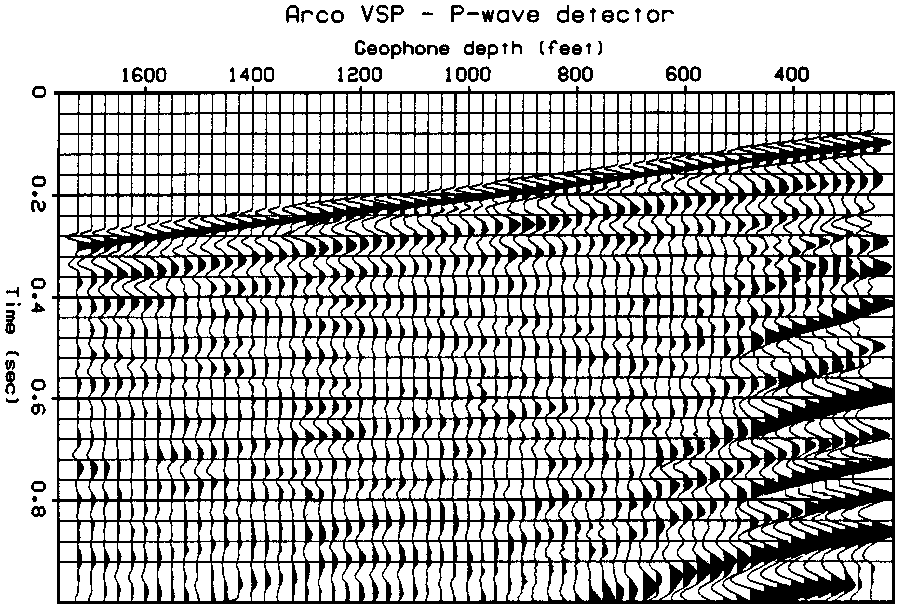
\includegraphics[width=0.65\textwidth]{mltp/vsp2}
% \caption[vsp2]{
% 图\ref{fig:mltp/vspl}的数据按浅层接收点增强而得的结果。振幅
% 均按$t^{1.5}$作比例标定(ARCO公司)
% }
% \label{fig:mltp/vsp2}
% \end{figure}

% 图\ref{fig:mltp/vspl}中第一个脉冲的能量大体可与其余脉冲能量相比拟,如果VSP的显示不采用
% $t^{1.5}$进行比例标定,其余能量就会小一些,但是既然地面反射资料通常都用某些这类比例标
% 定(往往是采用$t^2$
% ),这就使得从统计的角度谈论标定数据中的能量变得更有意义了。所
% 以,交混回响能量是大体可与初至能量相比拟的。

% 在近地表区域以下,下行波随深度而缓慢变化。我们现在要问:如将排列横向移动的
% 话,下行波究竟会变化多少。显然,钻井不会横向移动,因而我们将局限于仅是地面震源横
% 向移动情形下的记录数据。由于近地表变动往往在横向上迅速改变,我们也许要担心下行波
% 波形也是随炮点位置而迅速变化。炮点附近的交混回响同任何地面接收器附近的馄响是类似
% 重复的,最终组成的交混回响就是近炮点交混回响与近检波点交混回响二者的摺积。因此,
% 为获得对地面垲震数据进行反褶积时所需要的信息,VSP应当利用许多地面震源位置进行记
% 录。

% 可惜,这样的非零炮检距VSP资料难得采用。当石油生产下降因而打算采用费用昂贵的
% 二次回采方法时八VSP的成本费用相比起来就不会显得那么高了;
% VSP观测期间停止生产的
% 损失与未来的利润收益二者之间孰轻孰重是很容易掂量出来的。

% 再有,我们应当思考一下所谓“坏”资料的意义。地震数据每当高于周围环境微地震干
% 扰的水平时,一般总是可重复的。但是往往信号却毫无意义,空间相关对我们来说无
% 关轻重。大多数资料在较大时间时的情形都适于这样描述,出现的问题或许是下列这些:
% (1)下行波波形拖有一个很长的尾巴;(2
% )尾巴是地面位置的某种无序函数(chaotic function );(3
% )尾巴的能量超过第一个脉冲的能量。因此,由于下行波内有如此之多的
% 随机性,上行波必然是难以理解的。

% \subsection{深海多次皮---极地纬度的现象}
% \label{sec:5.5.4}

% 有一种经常引人注意的事,即,海底多次反射似乎大都只在极地纬度才是问题,难得在
% 赤道区域内出现。由于所根据的统计资料不多,这种观察也许有不妥之点,不过有两个理由
% 可以解释为什么这种观察窄可能成立,无论统计数字是否适当,它们每个都具有意义。

% 天然气往往可溶化于水,因而提高了凝固温度,在高压下尤其如此;当存在天然气时形
% 成的冰,称为天然气水化物(gas hydrate),因此,在液体海洋之下可能存在有圈闭于沉
% 积物之内的固体天然气水化物,该天然气水化物使沉积物的刚度増大,从而増强了多次反
% 射。

% 关于在极地纬度地区出现强多次反射的第二个理由一定与冰蚀作用有关。海洋底部普通
% 都是慢速沉积细粒物质的场所,这类新沉积的岩层均较柔软,故可形成弱多次反射波;但是
% 在极地纬度地区,冰川的冲蚀作用将沉积物搬运走了,在发生侵蚀的地方,新剥露出的岩石
% 比新近形成的沉积物强固坚硬。因此形成了较强的反射。

% 大陆在所有纬度上都会有侵蚀和沉积,然而,人们可以推测,在平衡时,在低纬度和中
% 等纬度地区的沉积作用形成了大陆斜坡,以后漂移至高纬度地区,在那里它们被侵蚀了。尽
% 管这很大程度上是推测想象,但这种理论确实为多次反射与极地纬度有关的原因提供了一种
% 解释。

% \subsection{微屈多次反射与层内多次反射}
% \label{sec:5.5.5}

% 所有多次反射类型均不出图\ref{fig:mltp/multpath}所示三类基本范畴之一。

% \begin{figure}[H]
% \centering
% 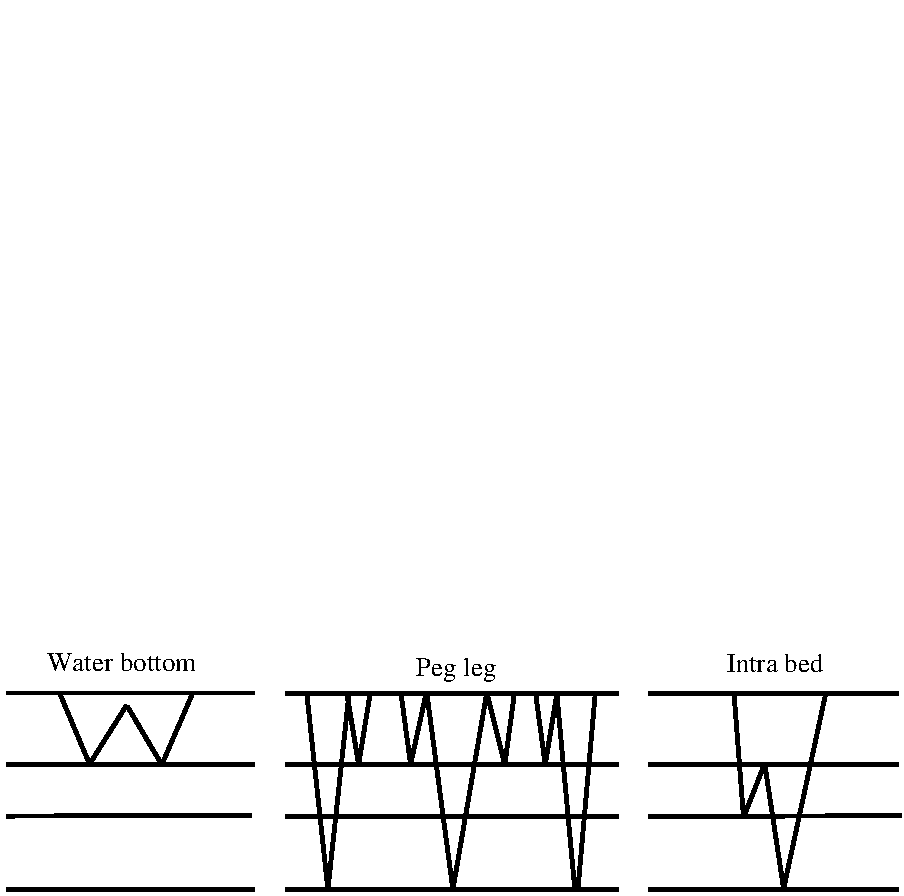
\includegraphics[width=0.65\textwidth]{mltp/multpath}
% \caption[multpath]{
% 所示射线路程分别为(a)海底多次波(b)微屈多次波(c)短程多次波
% }
% \label{fig:mltp/multpath}
% \end{figure}

% 海底多次波是射线路程整个位于海水层内部的那些多次波,如图\ref{fig:mltp/multpath}(a),由于海底通常
% 具有比深地质层位为高的反射率,海底多次波往往有很强振幅。在深水中,这些多次波可能
% 非常明显,截然不同,图\ref{fig:mltp/nearoffset}中所示是这类多次波的一个范例。

% \begin{figure}[H]
% \centering
% 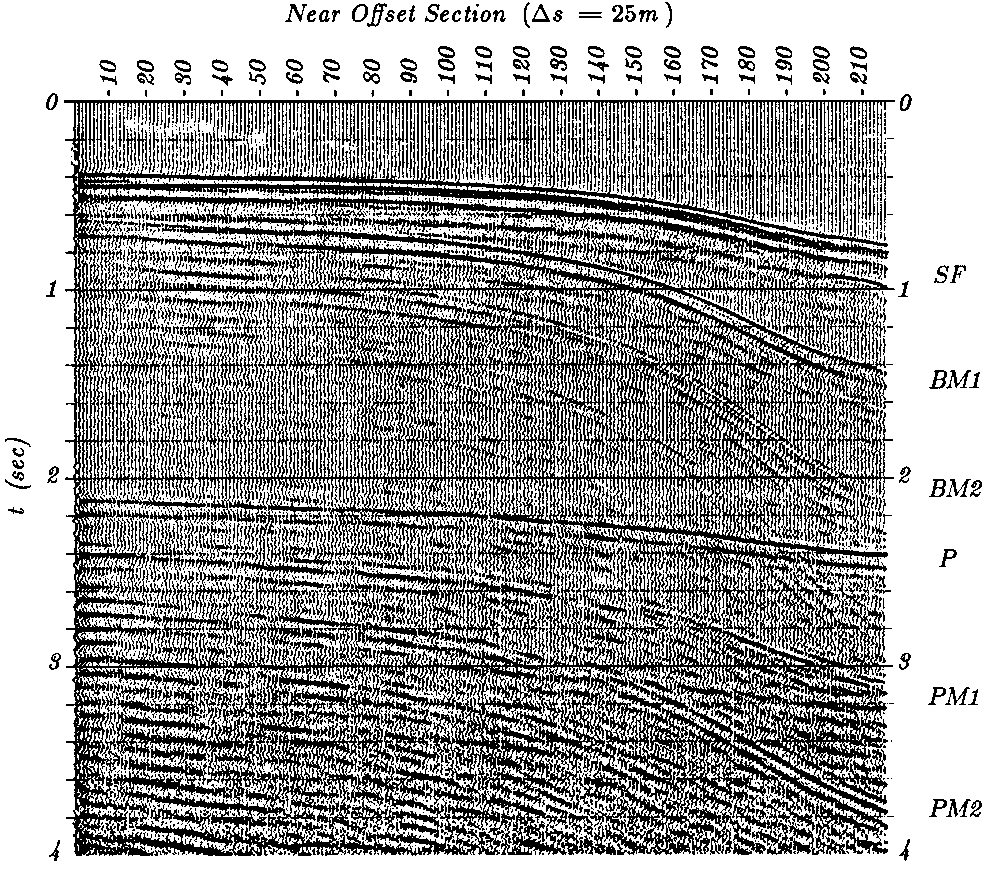
\includegraphics[width=0.65\textwidth]{mltp/nearoffset}
% \caption[nearoffset]{
% 近炮检距剖面---近海拉长石Flemish顶板岩层。
% 炮检距的距离约为9个炮点之距离,为海底,SF为第一个海底多次反射,BM2为第二个海底多次反
% 射。P为一次波,PMl为第一个微屈多次波,PM2为第二个微屈多次波(AMOCO-Canada公司)
% }
% \label{fig:mltp/nearoffset}
% \end{figure}

% 微屈多次反射按不同的作者有种种不同的定义,图\ref{fig:mltp/multpath}(b)中将微屈多次波定义为有
% 一次在沉积层系内发生反射而其他反射均在近地表发生的那些多次波。

% 为便于解释地震资料,让我们回顾一下层状介质内垂直入射多次反射的时间与振幅关
% 系。取海底反射系数为$c_1$,双程旅行时间为$t_1$,则第n次多次反射在时间$nt_1$到达,反射强度
% 为$c_1^n$;再假设较深层的一次反射旅行时间深度为$t_2$,具有反射系数$c_2$,于是海底微屈多次波
% 是在时间$t_2+nt_1$到达。注意,微屈多次波应成群到达,例如,时间$t_2+2t_1$可由三种路程所
% 形成,即$t_2+2t_1$、$t_1+t_2+t_1$或$2t_1+t_2$。因此,n阶微屈多次回声反射实际是来自n+1种射
% 线路程之反射的总和,从而其强度与$(n+1)c_2c_1^n$
% 成比例。海底混响的强度为这点同描述
% 沉积地层发生过一次反射混响时采用$(n+1)c_1^n$那样的n之函数是不相同的,忽略海底交混
% 回响本身,你可以仅把$(n+1)c_1^n$当作是爆炸波形。

% 每种多次波必然都有上行波变为下行波的“回车换向”点,儿乎所有容易识别的多次波
% 都是垲面多次波,就是说,它们的换向点均在地表,图\ref{fig:mltp/nearoffset}所示就是一些明显的例子,在
% 陆地勘探资料中,回车换向点可以是在土壤层底部,这差不多就同位于地表是一回事。

% 代表另一类称为“短程”多次波或“层内”多次反射波的射线路程,如图\ref{fig:mltp/multpath}
% (c)所
% 示,它们的换向点不在地表或不接近地表。在野外资料中,这类多次波极少是明显可见的,
% 尽管图\ref{fig:mltp/intrabed}所示是一种很清楚的情形,其中的这类多次波就不大容易看出来。它们能被追
% 踪识别,往往是因为地震资料是利用一些附带的测井记录进行综合解释的结杲,与微屈多次
% 波相比,这类短程多次波如此难以观察到的原因就在于:沉积层系内部的反射系数比自由面
% 上的反射系数低很多,不过,短程多次波的这个弱点可以被它们可能出现的次数非常之大所补
% 偿。不论任何时候,只要地震剖面变得难以解释,我们就可假定资料准是己变得以短程多次
% 波占压倒优势了。

% \begin{figure}[H]
% \centering
% 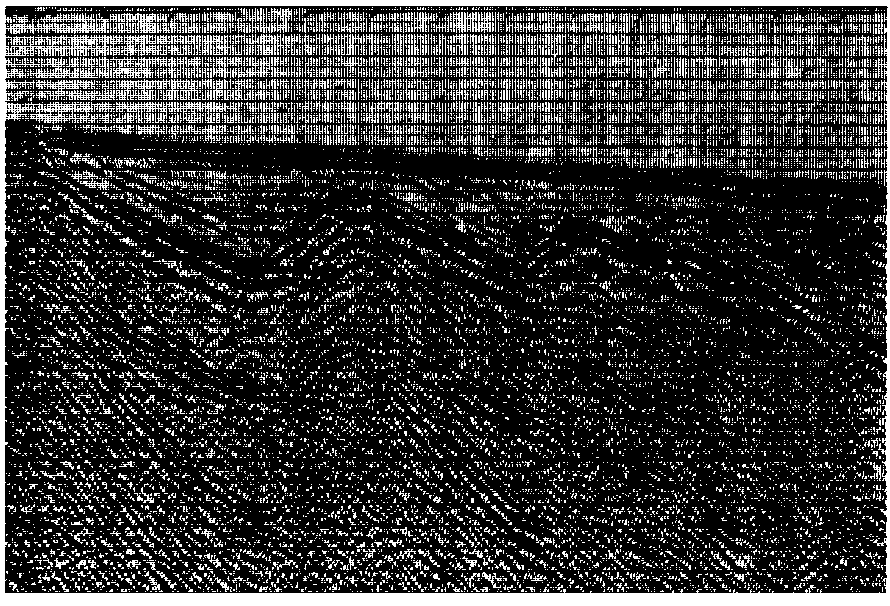
\includegraphics[width=0.65\textwidth]{mltp/intrabed}
% \caption[intrabed]{
% 有确凿之层间多次反射的罕有情形
% 资料系在波多黎各附近记录到,层内多次波处于海底反射与基底反射之间,因而其旅行时间为
% $t_{base}+(t_{base}-t_{floor})$,你看出它没有?(据西方地球物理公司)
% }
% \label{fig:mltp/intrabed}
% \end{figure}

% \subsection{对各种剖面类型需有所区别}
% \label{sec:5.5.6}

% 到1974年前后,波动方程方法业已证实是对共深度点叠如剖面进行偏移的成功途径,受
% 到这科成功的鼓舞,Don
% Riley和我开始把波动方程应用于深水多次反射的预测压制问题。
% 假定所遇到的一切困难之原因是绕射影响,现在又包括了深水多次反射影晌,我们发展了一
% 种用于模拟和预测消除绕射多次反射波的方法(参阅《地球物理数据处理基础》一书第11
% 章)。过去我们不理解在实际处理时绕射多次反射问题竟会比处理一次反射问题困难得多,对
% 于一次反射而言,相同的基本方法对零炮检距剖面、共深度点叠加剖面或垂直入射平面波剖面
% 等一视同仁都起作用,而我们的多次波压:制方法却证明仅能应用于垂直平面波叠加情形.
% 在Don
% Riley所提供的图\ref{fig:mltp/sections}中,对此作了一些比较。

% \begin{figure}[H]
% \centering
% 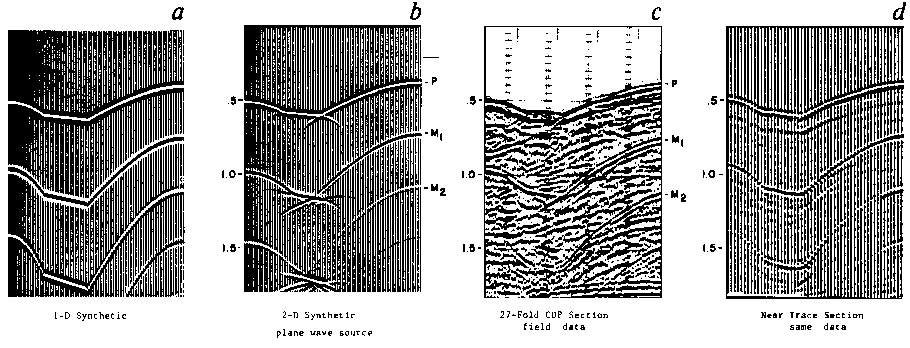
\includegraphics[width=0.65\textwidth]{mltp/sections}
% \caption[sections]{
% 绕射多次反射例子:(a)一维合成记录。(b)二维合成记录,垂直平面波震源。
% (c)27次覆盖CDP剖面。(d)近记录道剖面(据Riley)
% }
% \label{fig:mltp/sections}
% \end{figure}

% 研究图\ref{fig:mltp/sections}中的各种对照比较时要记住一件事,在野外资料上也许还识别不出来的似
% 乎就数三维形式的传播面貌了,这第三维次总像不可外扬的“家丑”一样,秘而不见,这
% 点通常并不妨碍二维偏移,但是可并未向我们保证它不会妨碍二维波动方程多次波压制方
% 法。

% \subsection{浅水多次波聚焦现象的例子}
% \label{sec:5.5.7}

% 爆炸反射面概念不能应用于多次反射,所以不存在什么可以在近记录道剖面上预测多次
% 波之聚焦冇为表现的简单波动理论手段工具。幸好垂直平面波叠加剖面中之多次波是可分析
% 的,它们能够给我们提供关于其他迪震剖面上多次反射之聚焦行为表现的某种概念。垂直下
% 行平面波可用无时差校正的共检波点叠加来模拟,这种共检波点叠加并不与熟悉的共深度点
% 叠加(CDP)相同,但却可用第一章与第二章中所述技巧对它进行分析。

% 试考虑一下经历过若干次由地面发生反弹的多次反射。一开始传播的时候,它是一个下行
% 平面波,如此保持不变,直至它由海底发生第一次反射。海底的反射使该平面波受到了海底
% 地形的影响,利用透镜项方程能在计算机内模拟地形对平面波的这种影响,这时由海底各点
% 形成绕射,向上传播至地面,然后又反射向下至海底,于是再应用透镜项方程在计算机内又
% 一次模拟出因海底地形影响而出现的时移。如此交错采用绕射和地形透镜时移
% (topographic lens shift)的过程能随你所愿地重复进行。图5.
% 5-10所示就是这样一种模拟结果,图\ref{fig:mltp/simulated}中的
% 高阶多次反射之突出特征是能量集中在局部化区域内,很容易看出海底凸出部分的反射如何
% 能够克服地震波能量扩散开来的趋势,时间坐标轴较深部位上出现的这些能量高度集中区完
% 全不像一次波,对一次波来说,局部化扰动应有扩散开来成为宽阔双曲线同相轴的趋向。如
% 若对图\ref{fig:mltp/simulated}中所见那些能量高度集中点像对一次波那样作偏移,必然是形成半圆弧形,这类
% 半圆弧形丝毫也不像是什么地质模型,而且即使采用生产应用上最佳的偏移程序处理,也完
% 全不会使结果有什么改变。

% 从图\ref{fig:mltp/simulated}的合成多次及射得到的最重要经验就是:多次波并不需要与一次波相似。偏
% 移叠加剖面上出现的半圆弧形同相轴可能是剩余多次反射,可惜,还没什么简单理论可以说
% 明垂直平面波叠加剖面上的聚焦多次波是否应
% 当类似于零炮检距剖面或CDP叠加剖面上的那
% 些多次波。幸亏还存在有可以提供答案的一些资料,图\ref{fig:mltp/multfoc2}是一个零炮检距剖面,它证实 在反射法勘探资料上如果不是以定量方式至
% 少也是以定性方式确实可以发现此类聚焦现象。

% 图\ref{fig:mltp/multfoc2}展示的海上勘探资料清楚地显示
% 出图\ref{fig:mltp/simulated}合成记录计算中的聚焦现象,这使
% 我们想到,为了得到清晰的地下界面图像,应
% 当以定量方式利用我们对此问题的理解。但是
% 有若干原因使我们作不到这点,第一,Riley
% 的理论只适用于垂直平面波叠加剖面,这些剖
% 面在定量上就不同于共中心点叠加剖面;第
% 二,地震剖面上海底的实在深度是未知数,它
% 必须根据数据资料本身以某种什么方法来确定;第三,图\ref{fig:mltp/simulated}中的海水深度太浅,以致各个单独反射无法加以区别。

% \begin{figure}[H]
% \centering
% 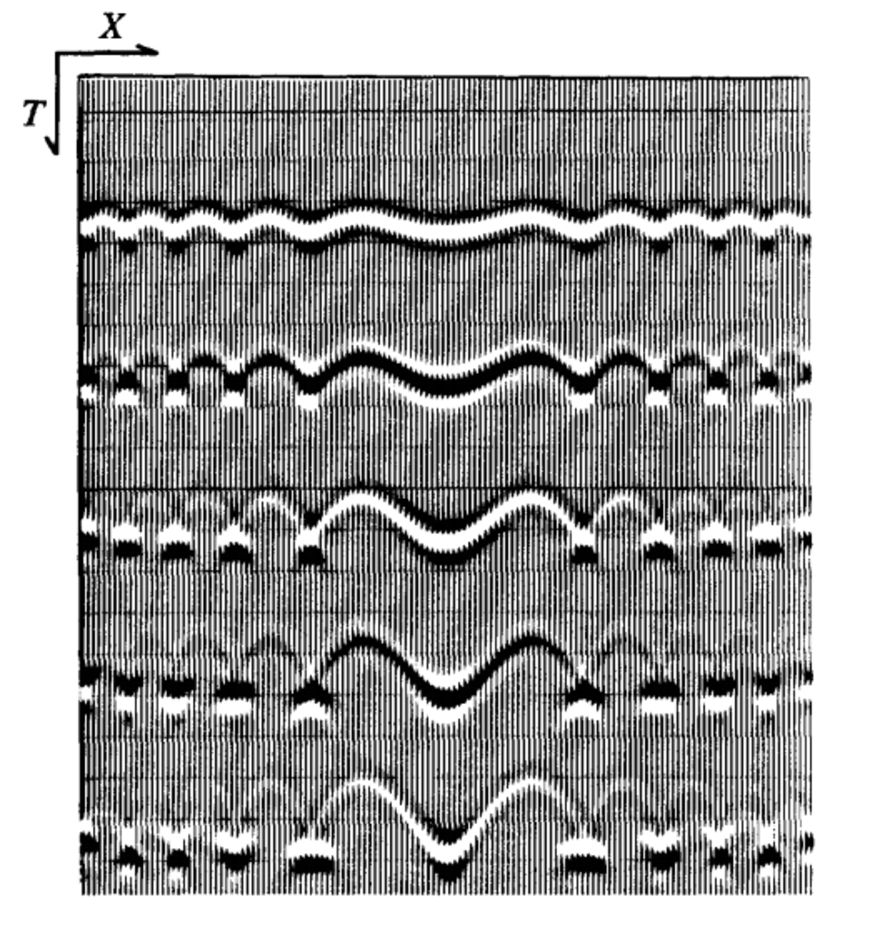
\includegraphics[width=0.65\textwidth]{mltp/simulated}
% \caption[simulated]{
% Chukchi海地区近记录道剖面中的聚焦作用对多次反射影响的例子,
% 这些影响为叠加所掩盖(据美国Geological Survey)。A. 现
% 存的构造;B. 以前的构造已不均匀侵蚀掉,留下海底的局部性
% 凸起或凹下;C. 高阶多次反射在海底凹下之处聚焦;D. 暴露在
% 多次波微弱之处(即海底凸出引起多次波迅速扩散之处)的时窗
% 内之现存构造倾角
% }
% \label{fig:mltp/simulated}
% \end{figure}

% \begin{figure}[H]
% \centering
% 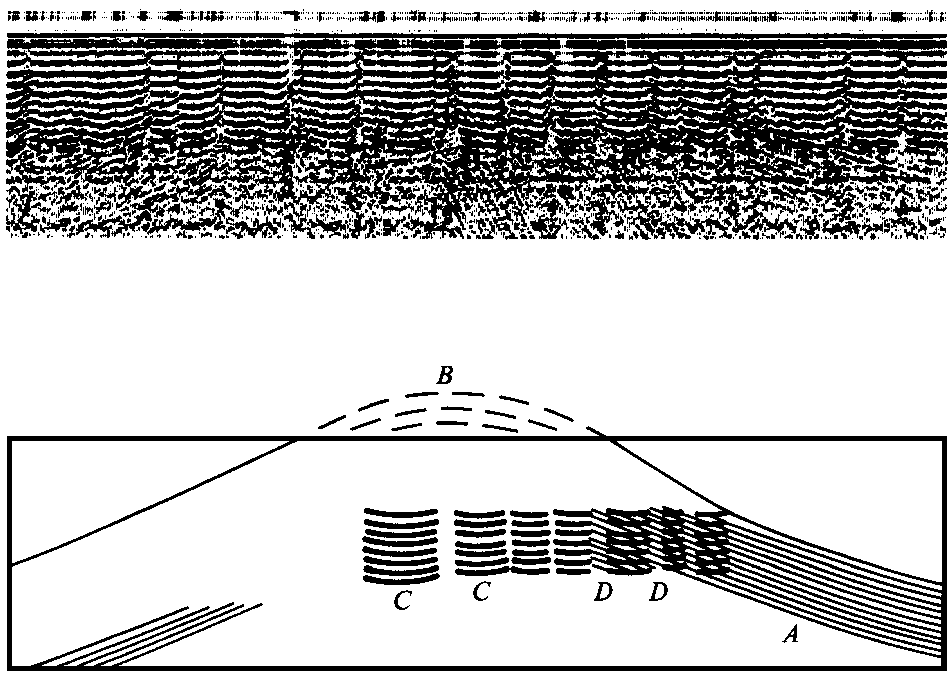
\includegraphics[width=0.65\textwidth]{mltp/multfoc2}
% \caption[multfoc2]{
% 绕射多次反射例子:(a)一维合成记录。(b)二维合成记录,垂直平面波震源。
% (c)27次覆盖CDP剖面。(d)近记录道剖面(据Riley)
% }
% \label{fig:mltp/multfoc2}
% \end{figure}

% \subsection{反褶积为何在深水情形下失败}
% \label{sec:5.5.8}

% 在深水情形下,反褶积处理一般是无效的,这已是众所周知的了。所以如此,有一个可
% 能原因,即深水条件并不是多次反射问题等价于爆炸波形问题的数学极限条件;不过,事情
% 还不完全仅限于此。

% 理论预言多次波在普通环境条件之下应有极性交错变化。图\ref{fig:mltp/multiple}和图\ref{fig:mltp/gsidecon}的例子证实
% 了这点,你也许已注意到,这种极性交错变化可能很难在CDP叠加资料中观察出来,但是在实
% 际工作中,如果条件顺利,还是容易观察到的。尽管图\ref{fig:mltp/nearoffset}的图幅较小,你在图中还是能
% 看出它的。在浅水中,各个脉冲到达时间太靠近,没法把它们区别开来;或者炮检距所张角
% 度成了掠射角,而理论预言在超过临界角时会有不同于$\pi$的相移,因此你在那种情形下见不
% 着简单的极性交错现象是理所应当的。在深水中,脉冲均彼此可区别,在最近的炮检距上应
% 可观察到极性交错,但是要在共中心点叠加剖面上寻找交错的极性,那你就会碰到麻烦,这
% 也就是用反褶积方法从共中心点叠加剖面中消除深水多次波为什么会趋于失败的原因。

% 回想一下各多次波在零炮检距上的时间关系。混响周期按说是常数,但因为有正常时
% 差,在任何其他炮检距上情形却并非如此。正常时差校正能成功地在恒定速度地层情形下恢
% 复零炮检距上的时间关系,但是在速度随深度而增大时,多次波所具有的均方根速会将比一
% 次波均方根速度低,因此,成问题的是采用什么速度以及在典型的陆地与海上勘探情况下剩
% 余时移是否大于半波长。回答这个问题不需要求解什么方程,只需全面观察常规共中心点叠
% 加能压制多次波就是因为多次波具有比一次波为低的速度,这种观察说明正常时差校正照例
% 是使多次波具有超出其自然零炮检距关系半个波长左右的时移。

% 我们所期望之零炮检距上的振幅关系出现混乱,会使事情变糟。反射系数是反射角度之
% 函数,可是从某个特定炮检距上的地震记录开始,各个多次反射就会已经是以不同的角度反
% 射的了。

% 垂直入射的时间关系是近似显示在共深度点叠加剖面上的,实际应用时的困难在于,共
% 深度点叠加模仿垂直入射情况还没完美到足以使人能够满意地从一次波预测出多次波。

% 在叠加以前,对海上资料可以采用海水速度完成时差校正,但这时任何微屈多次波就会
% 不适用于法线入射的时间关系了,既然微屈多次波是多次反射问题中最难处理的部分,也许
% 是应该以微屈多次波的速度来完成时差校正才好,不管你如何考虑这问题,反正所有深水多
% 次反射的时间关系严格说都不可能用时差校正的办法来调整。

% \subsection{习 题}
% \label{sec:5.5.9}

% \begin{enumerate}
% \item 在某种陆地勘探资料上已经注意到有这种现象,即深水多次反射到达时间比理论
% 所预言的时间要稍微早一点,试问这种现象应如何解释?
% \end{enumerate}